% 
% This message contains the LaTeX template for scribe notes
% in EE597.  You are free to use other means of producing
% your notes, but you are encouraged to use LaTeX: you will
% need to learn it some day.
% 
% Many thanks to Alistair Sinclair@cs.berkeley.edu for providing the basis for
% the first version of this template.
% 
% %************************************************************
%
% This is the LaTeX template file for lecture notes for EE596
% Pattern Recognition II: Introduction to Graphical Models.  When preparing 
% LaTeX notes for this class you must use this template.
%
% To familiarize yourself with this template, the body contains
% some examples of its use.  Look them over.  Then you can
% run LaTeX on this file.  After you have LaTeXed this file then
% you can look over the result either by printing it out with
% dvips or using xdvi.
%

\documentclass{article}
\usepackage{times,amsmath,amsthm,amsfonts,eucal,graphicx,amssymb}

% This scribe template not only uses latex, but also
% the American Mathematical Society (AMS) latex macros.
% Detailed documentation on how to use them to produce good
% math formating can be obtained here: http://www.ams.org/tex/
% I've also placed a copy of the AMS-Latex documentation
% on the web page at:
%     http://www.ee.washington.edu/class/596/patrec/scribes/amsguide_2p.ps
% Latex documentation can be obtained from 
%
% Publications related to latex are listed here:
%     http://www.ams.org/tex/publications.html
%

\setlength{\oddsidemargin}{0.25 in}
\setlength{\evensidemargin}{-0.25 in}
\setlength{\topmargin}{-0.6 in}
\setlength{\textwidth}{6.5 in}
\setlength{\textheight}{8.5 in}
\setlength{\headsep}{0.75 in}
\setlength{\parindent}{0 in}
\setlength{\parskip}{0.1 in}

%
% The following commands set up the lecnum (lecture number)
% counter and make various numbering schemes work relative
% to the lecture number.
%
\newcounter{lecnum}
\renewcommand{\thepage}{\thelecnum-\arabic{page}}
\renewcommand{\thesection}{\thelecnum.\arabic{section}}
\renewcommand{\theequation}{\thelecnum.\arabic{equation}}
\renewcommand{\thefigure}{\thelecnum.\arabic{figure}}
\renewcommand{\thetable}{\thelecnum.\arabic{table}}

%
% A few symbols that we will be using often in this course.
\newcommand{\indep}{{\bot\negthickspace\negthickspace\bot}}
\newcommand{\notindep}{{\not\negthickspace\negthinspace{\bot\negthickspace\negthickspace\bot}}}
\newcommand{\definedtobe}{\stackrel{\Delta}{=}}
\renewcommand{\choose}[2]{{{#1}\atopwithdelims(){#2}}}
\newcommand{\argmax}[1]{{\hbox{$\underset{#1}{\mbox{argmax}}\;$}}}
\newcommand{\argmin}[1]{{\hbox{$\underset{#1}{\mbox{argmin}}\;$}}}

%
% The following macro is used to generate the header.
%
\newcommand{\lecture}[4]{
   \pagestyle{myheadings}
   \thispagestyle{plain}
   \newpage
   \setcounter{lecnum}{#1}
   \setcounter{page}{1}
   \noindent
   \begin{center}
   \framebox{
      \vbox{\vspace{2mm}
    \hbox to 6.58in { {\bf CSC565 - Graph Theory
                        \hfill North Carolina State University} }
    \hbox to 6.58in { {\bf Fall 2019
                        \hfill Dept. of Computer Science} }
       \vspace{4mm}
       \hbox to 6.28in { {\Large \hfill Lecture #1: #2  \hfill} }
       \vspace{2mm}
       \hbox to 6.28in { {\it Lecturer: {\it Prof: Donald Sheehy {\tt <drsheehy@ncsu.edu>}} \hfill Scribe: #3} }
      \vspace{2mm}}
   }
   \end{center}
   \markboth{Lecture #1: #2}{Lecture #1: #2}
   \vspace*{4mm}
}

%
% Convention for citations is authors' initials followed by the year.
% For example, to cite a paper by Leighton and Maggs you would type
% \cite{LM89}, and to cite a paper by Strassen you would type \cite{S69}.
% (To avoid bibliography problems, for now we redefine the \cite command.)
% Also commands that create a suitable format for the reference list.
\renewcommand{\cite}[1]{[#1]}
\def\beginrefs{\begin{list}%
        {[\arabic{equation}]}{\usecounter{equation}
         \setlength{\leftmargin}{2.0truecm}\setlength{\labelsep}{0.4truecm}%
         \setlength{\labelwidth}{1.6truecm}}}
\def\endrefs{\end{list}}
\def\bibentry#1{\item[\hbox{[#1]}]}

%Use this command for a figure; it puts a figure in wherever you want it.
%usage: \fig{NUMBER}{CAPTION}{.eps FILE TO INCLUDE}{WIDTH-IN-INCHES}
\newcommand{\fig}[4]{
			\begin{center}
	                \includegraphics[width=#4,clip=true]{#3} \\
			Figure \thelecnum.#1:~#2
			\end{center}
	}
% Use these for theorems, lemmas, proofs, etc.
\newtheorem{theorem}{Theorem}[lecnum]
\newtheorem{lemma}[theorem]{Lemma}
\newtheorem{proposition}[theorem]{Proposition}
\newtheorem{claim}[theorem]{Claim}
\newtheorem{corollary}[theorem]{Corollary}
\newtheorem{definition}[theorem]{Definition}
% \newenvironment{proof}{{\bf Proof:}}{\hfill\rule{2mm}{2mm}}

% **** IF YOU WANT TO DEFINE ADDITIONAL MACROS FOR YOURSELF, PUT THEM HERE:

\begin{document}
%FILL IN THE RIGHT INFO.
%\lecture{**LECTURE-NUMBER**}{**DATE**}{**LECTURER**}{**SCRIBE**}
\lecture{12}{Oct 2, 2019}{Tanay Agrawal, Raj Shrivastava, Sreemoyee}
%\footnotetext{These notes are partially based on those of Nigel Mansell.}

% **** YOUR NOTES GO HERE:

% Some general latex examples and examples making use of the
% macros follow.  
%**** IN GENERAL, BE BRIEF AND COMPLETE. 


\section{Embeddings} % Don't be this informal in your notes!

\subsection{Introduction}

We recall that trees and forests have no $K_3$, which implies that they don't contain any cycles. Thus, we can say that trees and forests can be embedded into planes or we can obtain embedding of tree and forest graphs.

\subsection{Understanding Embedding}

In general, we can represent a graph G as:

$G = (V, E)$

The geometric realisation of G will be represented as:

$geom(G) \subseteq \mathbb{R}^n$

So, a continuous and injective mapping of this geometric realisation into a plane gives us an embedding of G, which can be denoted as:

$\underbar{G} \subseteq \mathbb{R}^2$

\textbf{Definition}: Faces are connected components of $\mathbb{R}^2 \smallsetminus \underbar{G}$
\begin{figure}[!h]
    \centering
    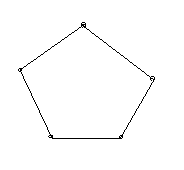
\includegraphics[width=0.3\textwidth]{images/fig1-12.png}
    \caption{A $C_5$ graph}
    \label{fig:C_5}
\end{figure}


The embedding for $C_5$ graph as shown in ~\ref{fig:C_5} has 2 faces.

\begin{figure}[h]
    \centering
    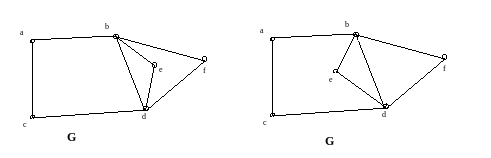
\includegraphics[width=0.9\textwidth]{images/fig2-12.png}
    \caption{Example of faces on graphs}
    \label{fig:fig2-12}
\end{figure}

The number of faces are same for both the left and right graphs but some of the faces from the embedding of these 2 graphs are different as they are formed using different cycles.

\subsection{Paths in graph and Topological spaces}

A path in a topological space is a continuous function from $[0,1]$ to space X, i.e., $f:[0,1] \longrightarrow X$

A path in a graph is some graph $P_m = (\{0,...,m\},\{i-1,i\} : i \in (1,...,m))$

As we can see that these two definitions of paths are closely related, i.e. an embedding of a path graph can be seen as a mapping into the interval $[0,1]$ (or can be seen as a path in linear space). The graph in ~\ref{fig:fig3-12} shows how a path graph $P_m$ can be visualised as an embedding into a topological space.

\begin{figure}[h]
    \centering
    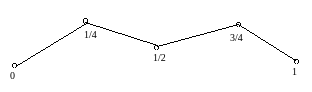
\includegraphics[width=0.55\textwidth]{images/fig3-12.png}
    \caption{Embedding of $P_m$ in topological space}
    \label{fig:fig3-12}
\end{figure}

\subsection{Linear embeddings}

Linear embedding maps straight lines to straight lines. It is defined as:

$M: \mathbb{R}^n \longrightarrow \mathbb{R}^2$  where M is a matrix, $M \in \mathbb{R}^{2xn}$

and if we define a point x as $x \in \mathbb{R}^n$

we get, $Mx \in \mathbb{R}^2$\\

\[
\begin{bmatrix}
    \dots   & x_{j}  & \dots  \\
    \dots   & y_{j}  & \dots  \\
\end{bmatrix}
b_{j}
=
\begin{bmatrix}
    x_{j}  \\
    y_{j}  \\
\end{bmatrix}
\]

\begin{figure}[h]
    \centering
    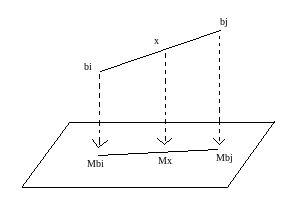
\includegraphics[width=0.5\textwidth]{images/fig4-12.png}
    \caption{A linear embedding of edge on plane}
    \label{fig:fig4-12}
\end{figure}

From the figure ~\ref{fig:fig4-12}, we understand that $x = \overline{{b_i}{b_j}}$

or, it an be written as a function of time as, $x = (1-t)b_i + tb_j$

Here, $b_i$ and $b_j$ are standard basis vectors. $b_i$ is a vector with all 0's in (n-1) positions and 1 in $i^{th}$ position. Consequently, $b_j$ is formed in same way.

Equivalently, $Mx = M((1-t)b_i + tb_j)$

or, $Mx = (1-t)Mb_i + tMb_j$

\subsection{Polygons}

A simple polygon is a linear embedding of $C_k$ (for some k).

Similarly, a polygon curve is a linear embedding of $P_m$.

\begin{figure}[h]
    \centering
    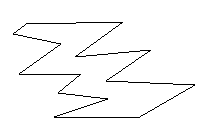
\includegraphics[width=0.5\textwidth]{images/fig5-12.png}
    \caption{A simple polygon: a linear embedding of $C_{14}$}
    \label{fig:}
\end{figure}

\section{Jordan Curve Theorem}
\subsection{Definition}
According to the (polygonal) Jordan Curve Theorem, every polygon P separates the plane into two pieces.
\subsection{J(x)}
In general, $J(x) = (\text{No. of crossings with a ray})$ mod 2

$J(x, r) = |ray(x, r) \cap P| \% 2 $ where $x \in \mathbb{R}^2\smallsetminus P$. 

This says that if x is any point inside or outside of any simple polygon P, then J(x) gives the number of intersections with P of a ray from x in the direction of r mod 2.

\begin{figure}[h]
    \centering
    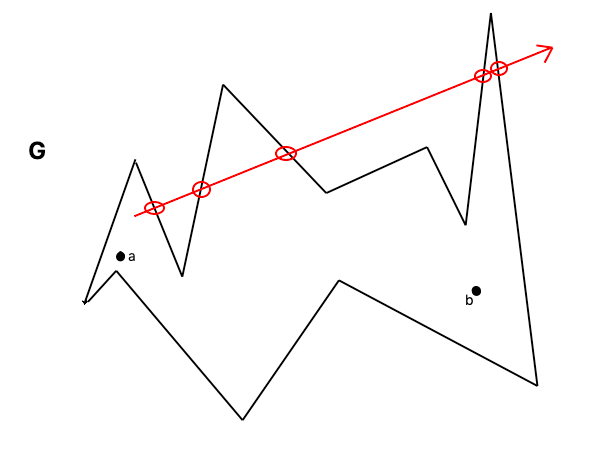
\includegraphics[width=0.5\textwidth]{images/jctSignificance.png}
    \caption{Significance of J(x)}
    \label{fig:jctSignificance}
\end{figure}

In Figure ~\ref{fig:jctSignificance}, it can be noticed that the total number of intersections of the ray r with the polygon P is always odd (called odd parity) when the ray begins from inside of the polygon and eventually emerges outside of the polygon or when it starts outside and emerges inside. Similarly, the total number of intersections is always even (called even parity) when the ray stays inside or outside of the polygon relative to where it began.\\

\subsection{Valid crossings}
Figure ~\ref{fig:validCrossings} illustrates few examples of valid and invalid crossings:
\begin{figure}[h]
    \centering
    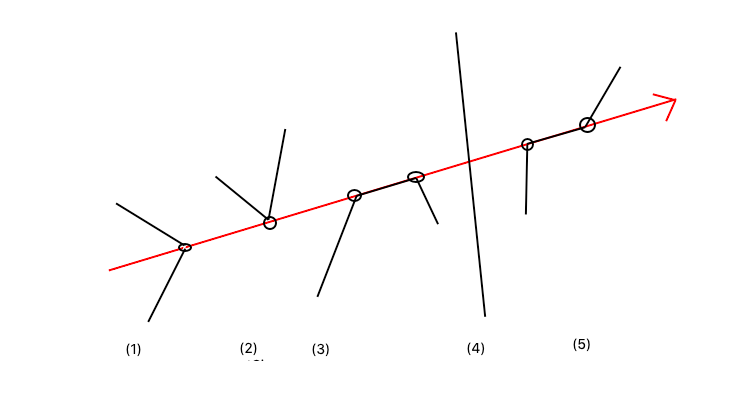
\includegraphics[width=0.45\textwidth]{images/validCrossings.png}
    \caption{Valid Crossings}
    \label{fig:validCrossings}
\end{figure}

In figure ~\ref{fig:validCrossings}, (1), (4) and (5) are valid whereas (2) and (5) are invalid crossings.

\subsection{Significance of the parity of number of crossings}
If we rotate the ray, the parity of the number of crossings remain the same before and after the rotation and is independent of the choice of the ray.

This can be illustrated by checking the parity of intersections of ray in different cases in Figure ~\ref{fig:validCrossings}.\\

\begin{table}[h]
\begin{tabular}{|l|l|l|}
\hline
\textbf{Case \#} & \textbf{Before crossing} & \textbf{After crossing} \\ \hline
\textbf{1}       & 1                        & 1                       \\ \hline
\textbf{2}       & 0                        & 2                       \\ \hline
\textbf{3}       & 2                        & 0                       \\ \hline
\textbf{4}       & 1                        & 1                       \\ \hline
\textbf{5}       & 1                        & 1                       \\ \hline
\end{tabular}
\end{table}

As clear from the table, the parity remains the same in all the five cases of figure ~\ref{fig:validCrossings}. 

\begin{theorem}
a and b are connected $\iff J(a) = J(b)$
\end{theorem}
\begin{proof}
1. a and b are connected $\implies J(a) = J(b)$\\
This can be proved by induction.\\
Say a, b are connected by a path of length m.\\
\textbf{Base}: one segment
\begin{figure}[h]
    \centering
    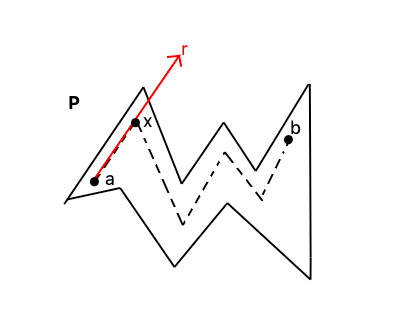
\includegraphics[width=0.37\textwidth]{images/jctProof1.png}
    \caption{Proof by induction}
    \label{fig:jctProof1}
\end{figure}
From figure ~\ref{fig:jctProof1}, ray (a, r) \textbackslash ray (x,r) = $\overline{ax}$\\
$\implies J(a) = J(x)$\\
\\\textbf{Induction step}: Path x to b has length of m - 1.\\
$\implies J(x) = J(b)\\$
\\So, J(a) = J(b)\\ 

2. J(a) = J(b) $\implies $ a and b are connected \\

\begin{figure}[h]
    \centering
    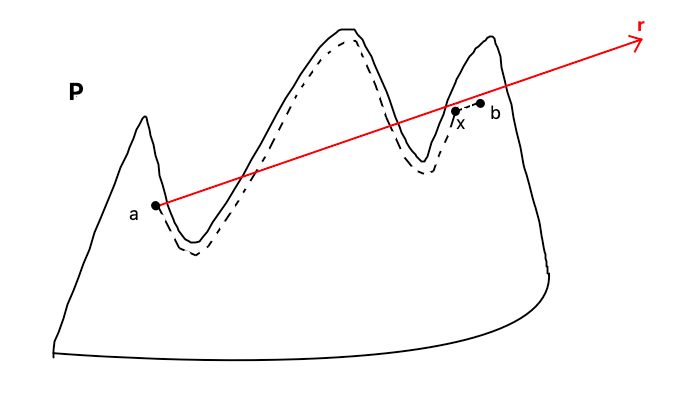
\includegraphics[width=0.4\textwidth]{images/jctProof2.png}
    \caption{Path along the edge of P}
    \label{fig:jctProof2}
\end{figure}

J(x) = J(a) \\
$\implies J(x) = J(b)$, since J(a) = J(b)\\
So, $\overline{xb} \subseteq \mathbb{R}^2$\textbackslash P
\end{proof}

\section{Face of graphs}
\subsection{Introduction}
\begin{figure}[h]
    \centering
    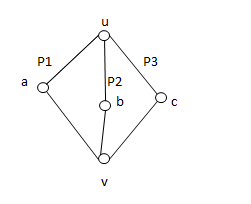
\includegraphics[width=0.4\textwidth]{images/Path_Image.PNG}
    \caption{Three disjoint paths from u to v}
    \label{fig:Path_Image}
\end{figure}

In figure ~\ref{fig:Path_Image}, there are 3 disjoint paths from u to v. Let us call them $P_1$, $P_2$, $P_3$. The $P_1 \cup P_2$ , $P_2 \cup P_3$ and $P_1 \cup P_3$ are the three faces of the graph. If we take any pair of these paths, we get a simple closed curve having an inside and a outside. $P_1 \cup P_3$ is an embedding of a circle and the path $P_2$ has to be either inside or outside of it. If we want to consider the vertex in $P_2$ to be outside, one of the other vertices has to lie inside.

\begin{figure}[h]
    \centering
    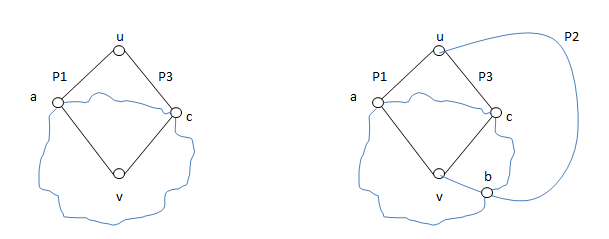
\includegraphics[width=0.6\textwidth]{images/Image_Proof.PNG}
    \caption{Identifying faces using Jordan curve}
    \label{fig:Path_Image}
\end{figure}

We draw two paths from a to c. One of them stays inside and the other outside. 
Together they form a Jordan curve.
Now, any path that goes to u to v has to cross one of these paths. 
Let us draw a path $P_2$ on the outside which crosses the Jordan curve at vertex B. 
We have now created a new Jordan curve with $P_1$ and $P_2$ which separates C from the
outer face. This is how we show that we cannot draw a graph like $K_{2,3}$ with all the vertices on the outer surface.
$K_4$ is also not outerplanar.

\subsection{Euler's Formula for the plane}
If G is an embedding then
$e(G) = |V_G| - |E_G| + |F_G|$ 
where $F_G$ is the number of faces in the embedding

\begin{theorem}
 $e(G) = 1 + |C_G|$ where $C_G$ is the number of connected components of the graph
\end{theorem}

\begin{corollary}
Since trees do not have any cycles, they have only one face. Hence, every drawing of a tree is a outerplanar embedding.
This is also true for a forest.
\end{corollary}

\begin{proof}
We perform induction on the number of edges. We first remove an edge and add the edge back in and observe what happens.\\
We keep a track of 4 different things - size of edge set, size of vertex set, number of faces and number of components.\\
$|V_G| - |E_G| + |F_G| = 1 + |C_G|$

We do not change the number of faces but we are reducing the number of components by 1.

Let us remove edge e(u,v) of the following Tree. Now, we can get the following cases:

Case 1: Faces on each side of e were the same.

$|F'| = |F|$ i.e. when the edge e is removed, the number of faces do not change. This means that around the edge, either sides were already connected. There was already a path as shown in the figure.

The Jordan curve separates the inside from the outside. So, the number of connected components has to go up when we remove the edge. 

So, there exists some polygon P separating the components. 

After removing the edge, $|C'| = |C_G| + 1$

$1 + |C| = |V| - |E| + |F|$

$2 + |C_G| = |V_G| - |E-1| + |F|$

\begin{figure}[ht]
    \centering
    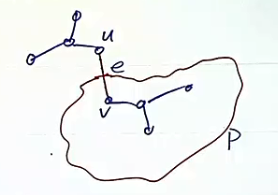
\includegraphics[width=0.5\textwidth]{images/Induction_trees.PNG}
    \caption{}
    \label{fig:Induction on trees}
\end{figure}

Case 2: Different faces on each side of e

$|F'| = |F| - 1$

In this case, e must have been part of a cycle surrounding one of the faces that separated it from the other one. If we look at that cycle, we find
another path from u to v which does not include e. Since there was already a path from u to v, number of connected components does not change.

$|C'| = |C|$
Therefore, faces and edges go down by one and the equation holds in this case too.
\end{proof}


% **** THIS ENDS THE EXAMPLES. DON'T DELETE THE FOLLOWING LINE:

\end{document}


